\documentclass[13pt]{extarticle}

\usepackage{graphicx,url}
\usepackage[portuguese]{babel}
\usepackage[utf8]{inputenc}
\usepackage{float}
\usepackage{setspace}
\usepackage{authblk}
\usepackage{datetime}

\usepackage{titling}

% autores na esquerda da página
\preauthor{\begin{flushleft}\large}
\postauthor{\par\end{flushleft}}

\usepackage{tabularx}
\usepackage{cite}
\usepackage{hyperref}

\usepackage{graphicx}
\usepackage{subcaption}
\usepackage{changepage}

%utilizar quadrados pretos no cronograma
\usepackage{xcolor}
\newcommand\crule[3][black]{\textcolor{#1}{\rule{#2}{#3}}}

\postdate{\end{center}\hspace*{-12.5em}}

\usepackage{tikzpagenodes}

% mudar tamanho do título do Abstract
\makeatletter
\renewenvironment{abstract}{%
    \if@twocolumn
      \section*{\abstractname}%
    \else
      \begin{center}%
        {\bfseries \Large\abstractname\vspace{\z@}}%  %% <- here I've added \Large
      \end{center}%
      \quotation
    \fi}
    {\if@twocolumn\else\endquotation\fi}
\makeatother

% logo do INCT
\newcommand{\mylogo}[1]{%
\tikz[remember picture,overlay] {%
  \node[inner sep=0pt,anchor=west] at ([yshift=0.05cm]current page text area.north west){#1};}
  }

% logo do IME (se precisar)
\newcommand{\usplogo}[1]{%
\tikz[remember picture, overlay] {%
	\node[inner sep=0pt, anchor=east] at ([yshift=0.05cm]current page text area.north east){#1};}
}

% margens
\usepackage[bottom=2cm,top=3cm,left=3cm,right=2cm]{geometry}


\usepackage{fancyhdr}
\pagestyle{fancy}

\usepackage{xcolor}


\begin{document}
\sloppy

\title{%
\huge \textbf{Projeto de Mestrado} \\~\\
  \Huge \textit{Identificação do projeto\\
  Quebrando linhas}\\
  \noindent\makebox[\linewidth]{\rule{\paperwidth}{0.5pt}}
  \LARGE \textbf{\textit{Identificação da instituição}}
  \noindent\makebox[\linewidth]{\rule{\paperwidth}{0.5pt}}
  \\~\\
  \Large Descrição com o número do processo e título\\
  }

\author{~\\~\\\textbf{Bolsista}\\Nome do Bolsista\\ Instituição\\~\\\textbf{Orientador}\\Nome do Orientador\\Instituição do Orientador\\~\\\textbf{Supervisor Tecnológico}\\Nome do supervisor tecnológico (se houver)\\Nome da Instituição\\}

\maketitle
\mylogo{
\includegraphics[scale=0.50]{images/Picture_interscity.png}} % imagem com o logo
\onehalfspacing
%-----------------------------------------------------------------------------%
\begin{abstract}

\begin{large}
  \begin{adjustwidth}{-1cm}{-1cm}
    Resumo do plano.
\end{adjustwidth}
\end{large}

\end{abstract}

\section{Introdução}
\label{sec:intro}

\begin{large}
  Texto de introdução do plano. Exemplo de citação: \cite{Babar2017}.
\end{large}

\section{Objetivos}

\begin{large}
Objetivo geral do plano.

Os objetivos específicos vão em seguida:
\begin{itemize}
  \item Objetivo específico 1
\end{itemize}
\end{large}

\section{Justificativa}
\label{sec:architecture}

\begin{large}
  Justificativa do plano
\end{large}

\section{Metodologia}
\label{sec:metodologia}

\begin{large}

  Exemplo de figura abaixo:

  \begin{figure}[ht]
  \centering
  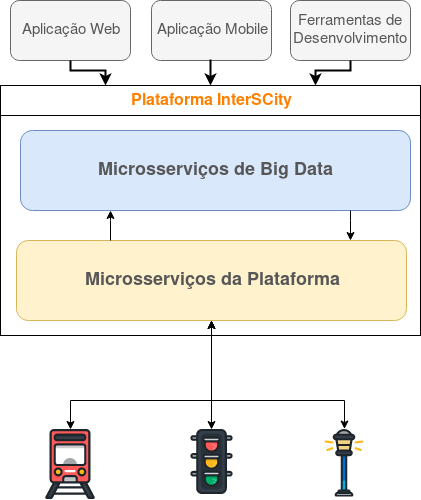
\includegraphics[scale=0.4]{images/interscity_platfor.png}
  \caption{Caption da imagem.}
  \label{fig:bigdataLayer}
  \end{figure}

\end{large}

\section{Atividades e Cronograma}
\label{sec:atividades}

\begin{large}

  Atividades do plano:

Demos início as seguintes atividades:
\begin{itemize}
\item Atividade 1;
\item Atividade 2;
\end{itemize}

Outras atividades, enumeradas:

\begin{enumerate}
	\item Atividade av1;
	\item Atividade av2;
\end{enumerate}

Exemplo de cronograma abaixo:

\setlength{\tabcolsep}{6pt}

\begin{table}[!htbp]
	\centering
    \scalebox{1}{
      \begin{tabular}{c|ccccccccccccccccccc}
      \hline
        &\multicolumn{18}{c}{Meses}\\
        \hline
        Atividades&1&2&3&4&5&6&7&8&9&10&11&12&13&14&15&16&17&18&19\\
        \hline
        \hline
        Atv. 1&\crule{0.3cm}{0.20cm}&\crule{0.3cm}{0.20cm}&\crule{0.3cm}{0.20cm}&\crule{0.3cm}{0.20cm}&\crule{0.3cm}{0.20cm}&\crule{0.3cm}{0.20cm}&\crule{0.3cm}{0.20cm}&\crule{0.3cm}{0.20cm}&\crule{0.3cm}{0.20cm}&\crule{0.3cm}{0.20cm}&\crule{0.3cm}{0.20cm}&\crule{0.3cm}{0.20cm}&\crule{0.3cm}{0.20cm}&\crule{0.3cm}{0.20cm}&\crule{0.3cm}{0.20cm}&\crule{0.3cm}{0.20cm}&\crule{0.3cm}{0.20cm}\\
        \hline
        Atv. 2&\crule{0.3cm}{0.20cm}&\crule{0.3cm}{0.20cm}&\crule{0.3cm}{0.20cm}&\crule{0.3cm}{0.20cm}&\crule{0.3cm}{0.20cm}&\crule{0.3cm}{0.20cm}&\crule{0.3cm}{0.20cm}&\crule{0.3cm}{0.20cm}&\crule{0.3cm}{0.20cm}&\crule{0.3cm}{0.20cm}&\crule{0.3cm}{0.20cm}&\crule{0.3cm}{0.20cm}&\crule{0.3cm}{0.20cm}&\crule{0.3cm}{0.20cm}&\crule{0.3cm}{0.20cm}&\crule{0.3cm}{0.20cm}&\crule{0.3cm}{0.20cm}&\crule{0.3cm}{0.20cm}\\
        \hline
        Atv. 3&&\crule{0.3cm}{0.20cm}&&&&&&&&&&\\
        \hline
        Atv. 4&\crule{0.3cm}{0.20cm}&\crule{0.3cm}{0.20cm}&\crule{0.3cm}{0.20cm}&\crule{0.3cm}{0.20cm}&&&&&&&&\\
        \hline
        Atv. 5&&&&&\crule{0.3cm}{0.20cm}&\crule{0.3cm}{0.20cm}&\crule{0.3cm}{0.20cm}&\crule{0.3cm}{0.20cm}&\crule{0.3cm}{0.20cm}&&&&\\
        \hline
        Atv. 6&&&&&&&&\crule{0.3cm}{0.20cm}&\crule{0.3cm}{0.20cm}&\crule{0.3cm}{0.20cm}&\crule{0.3cm}{0.20cm}&\crule{0.3cm}{0.20cm}&\crule{0.3cm}{0.20cm}\\
        \hline
        Atv. 7&&&&&&&&\crule{0.3cm}{0.20cm}&\crule{0.3cm}{0.20cm}&\crule{0.3cm}{0.20cm}&\crule{0.3cm}{0.20cm}&\crule{0.3cm}{0.20cm}&\crule{0.3cm}{0.20cm}&\crule{0.3cm}{0.20cm}&\crule{0.3cm}{0.20cm}\\
        \hline
        Atv. 8&&&&&&\crule{0.3cm}{0.20cm}&\crule{0.3cm}{0.20cm}&\crule{0.3cm}{0.20cm}&&&&&&\\
        \hline
        Atv. 9&&&&&&&&&&&&&&&\crule{0.3cm}{0.20cm}&\crule{0.3cm}{0.20cm}&\crule{0.3cm}{0.20cm}&\crule{0.3cm}{0.20cm}\\
        \hline
        Atv. 10&&&&&&&&&&&&&&&&\crule{0.3cm}{0.20cm}&\crule{0.3cm}{0.20cm}&\crule{0.3cm}{0.20cm}\\
        \hline
        Atv. 11&&&&&&&&&&&&&&&&&&&\crule{0.3cm}{0.20cm}\\
        \hline

      \end{tabular}
     }
\end{table}
\end{large}

%-----------------------------------------------------------------------------%
\bibliographystyle{splncs03}
\bibliography{referencias}
\end{document}
